\documentclass[conference]{IEEEtran}

%Template version as of 6/27/2024

\usepackage{cite}
\usepackage{amsmath,amssymb,amsfonts}
\usepackage{algorithm}
\usepackage{algorithmicx}
\usepackage{algpseudocode}
\usepackage{graphicx}
\usepackage{textcomp}
\usepackage{xcolor}
\def\BibTeX{{\rm B\kern-.05em{\sc i\kern-.025em b}\kern-.08em
		T\kern-.1667em\lower.7ex\hbox{E}\kern-.125emX}}
\begin{document}
	
	\title{Machine Learning 441 Assignment 2: Nearest Neighbours \& Decision Trees}
	\author{\IEEEauthorblockN{KT M\"ossner}
		\IEEEauthorblockA{
			26024284 \\
			26024284@sun.ac.za}
	}
	\maketitle
	
	\begin{abstract}
		The performances of two supervised machine learning classification algorithms are investigated in this report. The algorithms evaluated are $k$-nearest neighbours and classification trees, applied to the forest cover type dataset. The dataset contains several data quality issues that the machine learning algorithms are either sensitive or robust to. Specific data pre-processing was applied for each algorithm to address these data quality issues, without performing unnecessary pre-processing. Then, hyper-parameter tuning using cross-validation, model training on the training dataset and evaluation on the test dataset with multiple performance metrics. Analysis of results showed that the $k$-nearest neighbours algorithm with $k=3$ and the distance metric set to 'euclidean' had better cross-validation performance on the training set. However, the classification tree with entropy based splits and no maximum depth had better generalisation performance on the test dataset. Statistical analysis using the Wilcoxon signed-rank test confirmed that the observed performance differences between the models were significant. The findings outlined in this report conclude that classification trees were better suited for the forest cover type classification problem.
	\end{abstract}
	
	\section{Introduction}
	Classification algorithms are supervised machine learning techniques that are used to classify unseen observations into predefined classes based on patterns learned from training data.Machine learning classification algorithms encompass a wide variety of approaches. Different algorithms are better suited to different classification problems. The algorithms considered in the current assignment are the $k$-nearest neighbours ($k$-NN) and decision tree classification algorithms. The dataset that was considered for the classification problem is the forest cover type dataset, which contains observations from four areas of the Roosevelt National Forest in Colorado. This dataset includes various information on tree type, shadow coverage, distance to nearby landmarks, soil type, and local topography. The problem is to classify each observation into one of seven forest cover types, namely spruce/fir, lodgepole pine, ponderosa pine, cottonwood/willow, aspen, douglas-fir, or krummholz.
	
	The main objectives of this assignment consist of: identifying and addressing the data quality issues that are relevant in the forest cover type dataset; developing, implementing and optimising the two predictive models, namely the $k$-NN and classification tree algorithms; and lastly comparing the results of each classification algorithm to conclude which of the approaches is best for the problem.
	
	The forest cover type dataset contains several data quality issues, including missing values, highly correlated features, noisy features, outliers, features with large numeric ranges, mixed feature types, features with a cardinality of one, features with unique values, and skewed class distributions. The $k$-NN and classification tree algorithms are sensitive to specific data quality issues and robust to others. An example of this is the sensitivity of the $k$-NN algorithm to missing values whereas the classification tree algorithm is robust to this data quality issue. As a result of this only necessary data pre-processing procedures were applied before training the predictive models. 
	
	Once the necessary data pre-processing has been applied, the models are trained and evaluated using the cleaned datasets. In this implementation techniques such as cross-validation, training-test splits, hyper-parameter tuning, evaluation metrics and statistical tests were all applied to compare the performances of the algorithms. 
	
	The next section of this report gives a comprehensive overview and background of the $k$-nearest neighbours and classification tree algorithms, as well as the expectations regarding the impact that the data quality issues will have on each algorithm. Section \ref{M} provides a detailed description of the methodology followed to train the predictive models and generate predictions. Section \ref{EP} consists of the detailed data pre-processing procedures, the hyper-parameter tuning strategies, the performance metrics implemented, and the analysis process. The results from the predictive models are discussed in section \ref{RR} and the final conclusion of the key findings and their implications for forest cover prediction are presented in section \ref{C}.
	
	\section{Background}\label{B}
	\subsection{$k$-Nearest Neighbours}
	The $k$-nearest neighbour algorithm is a similarity based algorithm that requires two fundamental components: a feature space representation of the instances in a dataset and a measure of similarity between instances \cite{b1}. The $k$-NN algorithm is used for both classification and regression problems. The $k$-NN classifier is used to classify instances by assigning the observation to the class that is most common among its $k$ nearest neighbours ($k$ is a positive integer). The $k$-NN regression algorithm predicts values by averaging the target value of an instances $k$-nearest neighbours.
	
	Algorithm~\ref{alg:knn} provides a pseudocode definition of the $k$-NN classification algorithm that classifies a data point $\boldsymbol{x}$ given the dataset $D$ and a value of $k$. The algorithm loops over each data point $\boldsymbol{x}_i$ in the dataset and calculates the distance between this data point and $\boldsymbol{x}$. The distances for each data point is collected and sorted in ascending order. $S$ becomes the set consisting of the $k$ nearest neighbours of data point $\boldsymbol{x}$. The majority class for the data points in the set $S$ is determined and returned by the algorithm.
	\begin{algorithm}[H]
		\caption{k-Nearest Neighbors (kNN)}
		\begin{algorithmic}[1]
			\Function{kNN}{$D, \boldsymbol{x}, k$}
			\ForAll{$\boldsymbol{x}_i \in D$}
			\State $\boldsymbol{d} \gets \text{distance}(\boldsymbol{x}_i, \boldsymbol{x})$
			\EndFor
			\State sort($\boldsymbol{d}$)
			\State $S \gets$ set of $k$ nearest patterns to $\boldsymbol{x}$
			\State \Return majority class in $S$
			\EndFunction
		\end{algorithmic}
		\label{alg:knn}
	\end{algorithm}
	The value of $k$ has a large impact on the $k$-NN algorithm. Lower values of $k$ result in an unstable model with high variance and low bias, leading to an overfit model. Larger values of $k$ result in a model with low variance and high bias, where the model is more stable but more likely to be underfit.
	
	The best value for $k$ is problem and data dependent and it is best obtained through hyper-parameter tuning such as cross-validation. A simple heuristic to determine the value of $k$ is to set $k=\sqrt{N}$ where N is the number of observations. The value of $k$ determines how the $k$-NN algorithm is effected by outliers with smaller values of $k$ being less effected but more influenced by noise and larger values of $k$ being more influenced by outliers but more robust to noise. If the dataset contains outliers then smaller values of $k$ are more suitable. 
	
	The $k$-NN algorithm is sensitive to skew class distributions as the majority class will begin to dominate the nearest neighbours as $k$ increases. There are multiple different similarity and distance measures that are used with the $k$-NN algorithm. These measures apply to both numerical descriptive features and categorical descriptive features. To measure similarity between mixed feature types either convert the categorical features to numerical features and apply numerical similarity measures or compute a weighted sum between the numerical and categorical similarity measures. The $k$-NN algorithm can be applied to a wide variety of data types including image data, temporal times series data and text data. Selecting appropriate similarity measures for certain data types allows the $k$-NN algorithm to be applied to non-tabular data.

	\subsection{Classification Trees}
	Classification trees are non-parametric supervised machine learning models that are used to classify data points into predefined classes. Classification trees are a type of decision tree. Decision trees consist of a single root node, non-terminal nodes and terminal nodes that are connected by branches \cite{b1}. Decision trees form a tree structure with non-terminal nodes representing decisions based on the descriptive features and terminal nodes representing the target feature predictions. Each of the branches from a non-terminal node represent a single decision that has been made regarding a descriptive feature. 
	
	The prediction process of a classification tree begins by testing the value of a descriptive feature at the root node. The result of this test decides which branch to take to the next non-terminal node. This process is repeated until a terminal node in the tree has been reached and the value of the node is returned as the class prediction. Classification trees are also used to extract the production rules which describes how the model came to its decision. The classification tree is induced by the divide and conquer method where the training set is recursively split into smaller subsets of less inhomogeneity. This process is repeated until a specified stopping condition is met. The simplest stopping condition is to continue until all subsets are homogeneous, however this approach leads to deeper trees that are more likely to overfit the dataset. 
	
	Algorithm~\ref{alg:dt} provides the pseudocode for the induction of a classification tree, given some dataset $D$ with the stopping condition of homogeneous subsets. If the dataset is empty the default class is returned. If the dataset is homogeneous then return the class label for the dataset $D$. Otherwise $D$ is not homogeneous and is recursively split into $O$ number of outcomes based on a single descriptive feature. 
	\begin{algorithm}
		\caption{InduceTree}
		\begin{algorithmic}[1]
			\Function{InduceTree}{$D$}
			\If{$|D| = 0$} \Comment{$D$ is empty}
			\State \Return leaf with default class
			\EndIf
			\If{$|D| > 0$ \textbf{ and } $\forall \boldsymbol{x} \in D$ the class is the same, i.e. $y_m$} \Comment{$D$ is homogeneous}
			\State \Return leaf with class label $y_m$, containing $D$
			\EndIf
			\State Select a test based on a single descriptive feature
			\State Split $D$ into $D_1, D_2, \ldots, D_O$, where $O$ is the number of outcomes
			\For{$o = 1$ \textbf{to} $O$}
			\State \Call{InduceTree}{$D_o$}
			\EndFor
			\EndFunction
		\end{algorithmic}
		\label{alg:dt}
	\end{algorithm}
	The split of a descriptive feature is chosen to maximise the reduction in heterogeneity of the dataset. Entropy is the measure of homogeneity ranging between 0 and 1, with 0 representing perfect homogeneity in the dataset and 1 representing perfect heterogeneity. The formula for entropy is:
	\begin{equation}
		H(D)=-\sum^M_{m=1}p(y_m)\log_M p(y_m) \label{entropy}
	\end{equation}
	where the probability of a class $y_m$ occurring in $D$ is given as:
	\begin{equation}
		p(y_m)= \frac{\text{freq}(y_m, D)}{|D|}\label{classprob}
	\end{equation}
	$M$ is the number of classes and $\text{freq}(y_m, D)$ is the number of times class $y_m$ appears in dataset $D$.
	The measure of entropy for a given split is defined as:
	\begin{equation}
		H_x(D)  \sum^O_{o=1} p_o H(D_o) \label{entropy_split}
	\end{equation}
	where $x$ is the feature split on, $O$ is the number of outcomes resulting in subsets $D_1, D_2, ... D_O$ and $p_o$ is the probability of outcome $o$.
	The information gained based on a split for dataset $D$ on feature $x$ is be determined using both \eqref{entropy} and \eqref{entropy_split}:
	\begin{equation}
		\text{gain}(x)=H(D)-H_x(D) \label{gain}
	\end{equation}
	The information gain is a measure of how much more homogeneous the dataset would be if it was split on feature $x$. The objective of the classification tree is to maximise the information gain. The problem with information gain is that it favours variables with multiple outcomes which results in a higher branching factor and a more complex model. A solution to this problem is to normalise the information gain with entropy with respect to test outcomes:
	\begin{equation}
		\text{gainRatio}(x)=\frac{\text{gain}(x)}{\text{splitinfo}(x)} \label{gainratio}
	\end{equation}
	where $\text{splitinfo}(x)=-\sum^O_{o=1}p_o\log_Op_o$. The objective then becomes to select a descriptive feature $x$ that maximizes the gain ratio in \eqref{gainratio}.
	
	To prevent overfitting in classification trees the nodes of the tree are pruned to reduce the complexity of the model. Deeper level non-terminal nodes are replaced by terminal nodes. Subsets associated with test's terminal nodes are combined using a majority weighting scheme. The pruning process is continued while the generalisation performance increases and stops when it decreases. Classification tree pruning helps make the predictive model more robust to outliers and noise. Classification trees are sensitive to skew class distributions with minority classes resulting in small terminal nodes that are likely to be pruned.
	
	\subsection{Impact of Data Quality Issues}
	The forest cover type dataset contains multiple data quality issues that the $k$-nearest neighbours and classification trees (CT) classifiers are sensitive to:
	\begin{itemize}
		\item \textbf{Missing values}  
		\begin{description}
			\item [$k$-NN:] The $k$-NN algorithm is sensitive to missing values and the model cannot be trained with missing values in the dataset. The solution is to impute the missing values if possible otherwise ignore the missing values in the distance calculation.
			\item [CT:] Classification tree induction algorithms are capable of dealing with missing values. The calculation of the gain ratio when conducting a test on a descriptive feature $x$ becomes:
			$$
			\text{gainRatio}(x) = (1 - F)(H(D) - H_x(D))
			$$ 
			where $F$ is the fraction of patterns in the dataset $D$ for which the value of $x$ is missing. To classify patterns with missing values, a class distribution is computed and the class with the highest probability is selected.
		\end{description}
		
		\item \textbf{Feature correlation}  
		\begin{description}
			\item [$k$-NN:] Correlated features provide redundant information but still contribute to distance measures, therefore distorting the distance measures. This adds noise to the algorithm and makes it more difficult to identify the nearest neighbours.
			\item [CT:] Classification trees are robust to feature correlation since the algorithm selects one feature at a time to split on.
		\end{description}
		
		\item \textbf{Noisy features}  
		\begin{description}
			\item [$k$-NN:] $k$-nearest neighbour's sensitivity to noise depends on the value of $k$. A smaller value of $k$ leads to overfitting in the $k$-NN algorithm and is therefore sensitive to noise. A larger value for $k$ leads to more generalisable model and is less sensitive to noise.
			\item [CT:] Classification trees are robust to noisy features. Noisy patterns will be pruned away and will not affect the majority class.
		\end{description}
		
		\item \textbf{Outliers}  
		\begin{description}
			\item [$k$-NN:] The effect that outliers have on the $k$-NN algorithm depends on the value of $k$. For smaller values of $k$ the outliers are not likely to be the nearest neighbours as they are further away and will not have an influence on the predicted value. For larger values of $k$, outliers have an influence on the predicted value as more neighbours are considered for the predicted value. The influence of the outliers however is limited due to the majority voting being used.
			\item [CT:] Classification trees are robust to outliers as they will be pruned away in the terminal nodes just as the noisy features are.
		\end{description}
		
		\item \textbf{Features with significantly differing numeric ranges}  
		\begin{description}
			\item [$k$-NN:] Features that have large numerical range values will have a stronger impact on the distance calculations than small range values. It is important to scale all of the input features to the same range.
			\item [CT:] Classification trees are robust to significantly differing numeric ranges as the splits for descriptive features are based on specified thresholds and not distances.
		\end{description}
		
		\item \textbf{Numerical and categorical features}  
		\begin{description}
			\item [$k$-NN:] $k$-nearest neighbours is robust to datasets with numerical and categorical features by using similarity measures that work for both feature types such as the Gower similarity metric. Alternatively the categorical features are converted into numeric features and a similarity measure for numerical features is applied. 
			\item [CT:] Classification trees naturally handle both categorical and numerical descriptive features by sorting the numeric features, performing splits on each numerical value and evaluating the information gain for each split.
		\end{description}
		
		\item \textbf{Feature with cardinality of one}  
		\begin{description}
			\item [$k$-NN:] Provides no additional information to the $k$-NN algorithm.
			\item [CT:] This data quality issue will have no effect on the classification tree algorithm. This feature will never be chosen for splitting by the classification tree algorithm since there is no unique values to split on.
		\end{description}
		
		\item \textbf{Feature with unique value for each observation}  
		\begin{description}
			\item [$k$-NN:] Unique values severely distort the distance calculations and therefore make other features irrelevant.
			\item [CT:] Classification trees that use the information gain ratio are robust to unique values as the information gain ratio penalizes features with many outcomes to move lower in the classification tree. These features will subsequently be removed during the post-pruning process.
		\end{description}
		
		\item \textbf{Skewed class distributions}  
		\begin{description}
			\item [$k$-NN:] Sensitivity of the $k$-NN algorithm to skewed class distributions depends on the value of $k$. As the value of $k$ increases the majority class will dominate the nearest neighbours of observations. Smaller values for $k$ are more robust to skewed class distributions. 
			\item [CT:] Classification trees are sensitive to skewed class distributions. The instances from the minority classes are going to result in small terminal nodes that are likely to be pruned and the the instances combined to form a subset for the parent node will be classified as the majority class.
		\end{description}
	\end{itemize}

	\section{Methodology}\label{M}
	The methodology followed in this assignment discusses how the problem was approached, implemented and solved. The $k$-NN and classification tree algorithms were both implemented using the Scikit-learn library \cite{b3}. The \texttt{KNeighborsClassifier} was used for the $k$-NN classification algorithm and the \texttt{DecisionTreeClassifier} was used for the classification tree. Both machine learning models were trained using the forest cover type dataset stored as Pandas  DataFrames \cite{b2}. Each feature of every observation was represented using the NumPy \cite{b4} data types. Prior to the model training, necessary data pre-processing procedures were applied to the dataset. Separate data pre-processing procedures were considered for each classification algorithm. Two copies of the original dataset were made to ensure that no unnecessary data pre-processing was implemented. This approach was followed to ensure that only algorithm-specific data quality issues were removed for the respective classification algorithms. A comprehensive description of the data pre-processing that was implemented is provided in section \ref{EP}. 
	
	Once the data pre-processing procedures have been implemented, the dataset was split into a training and test set. The training dataset consists of 70 percent of the observations and the test set consists of the remaining 30 percent of the observations. The dataset was randomly shuffled before it was split into the training and test set. The training and test sets were stratified so that the ratio between target class labels in each split are consistent. This ensures that no class is under or over represented in the training and test sets.
	
	
	The \texttt{KNeighborsClassifier} and \texttt{DecisionTreeClassifier} algorithms require optimal hyper-parameters in order to extract the best performance from these machine learning models. Hyper-parameters are parameters that are set before the model is trained and effects how the algorithms learn from the data. Hyper-parameters that are not correctly tuned will result in models that underfit or overfit to the data. The hyper-parameters that were considered for the final trained models were determined by $k$-fold cross-validation. The $k$-fold cross-validation algorithm splits the training dataset into $k$ partitions and uses $k$-1 partitions as the training set and one partition as the validation set in the model training process. This process is repeated $k$ times with the validation set changing to a different partition each time. The average score of each trained model is the cross-validation score. The optimal set of hyper-parameters for each algorithm was determined by systematically evaluating multiple candidate values. This procedure, known as grid search cross-validation, uses a grid of possible hyper-parameter values to identify the configuration that results in best model performance. Once the optimal hyper-parameters were determined for each algorithm, the models were retrained on the full training datasets. 
	
	
	The performance of each model was evaluated on the test set by generating label predictions for the target class. The performance metrics chosen for the model evaluation were accuracy, precision, recall, F1-score, Cohen's kappa and Matthew's correlation coefficient. Multiple independent runs of the algorithms were conducted to evaluate the performances on the test dataset. The results for each run were generated by running the algorithms on a sample of the test dataset. The samples were created by splitting the test dataset into 20 stratified folds, which provided results for 20 independent runs. The results for each fold were observed and recorded for further analysis.
	
	\section{Empirical Procedure}\label{EP}
	Due to the fundamental differences between the $k$-nearest neighbours and classification tree algorithms, separate empirical procedures were implemented for each algorithm. Although both of these predictive models are used to solve the same classification problem, they are sensitive to separate data issues and they have different hyper-parameters used for model training. The following subsections explain the data pre-processing and hyper-parameter tuning procedures followed for each algorithm in detail:
	
	\subsection{$k$-Nearest Neighbours}
	\paragraph{Data Pre-processing}
	A copy of the original dataset is made before applying any of the data pre-processing. The missing values were imputed using the \texttt{SimpleImputer} from the Scikit-learn library, using a mean imputation method. The mean imputation method was chosen for the feature with missing values as it did not contain any outliers that would skew the mean calculations. The \texttt{\textbf{Facet}} feature was removed due to its high correlation with the \texttt{\textbf{Aspect}} feature. This feature provides redundant information in the predictive process and distorts the distance measures used in the similarity calculations. The noisy feature \texttt{\textbf{Inclination}} was removed as small values of $k$ lead to overfitting, and are therefore sensitive to noise. The severe feature values outliers were removed, (values beyond $\text{Q1} - 3\times\text{IQR}$ or $\text{Q3} + 3\times\text{IQR}$). The \texttt{\textbf{Water\_Level}} feature with a cardinality of one was removed, as well as the \texttt{\textbf{Observation\_ID}} feature for having unique values which would distort the distance metrics. 
	
	The dataset was split into a train-test split, with 70 percent of the observations chosen for the training set and 30 percent for the test set at random, with the random state set to 42. The training and test dataset split was stratified to preserve the class distributions of the target variable in both sets. All of the features of the forest cover type dataset were scaled to have zero mean and unit variance. The \texttt{StandardScaler} was fit to the training dataset and then used to scale the training and test datasets. 
	
	The class imbalances for the target variable was addressed by synthetically oversampling the minority classes with the SMOTE algorithm. Then the Tomek links algorithm was applied to undersample the majority class and clean up the decision boundary between classes. The \texttt{SMOTETomek} algorithm, from the \texttt{Imbalanced-learn} library \cite{b5}, was applied with the random state set to 42. A sampling strategy was specified so that the number of observations for each minority class was oversampled to 30\% of the size of the majority class. After applying synthetic oversampling to the training dataset, which consisted of 406,708 observations and 58 descriptive features, the final semi-balanced training dataset consisted of 633,819 observations and 54 descriptive features.
	
	\paragraph{Hyper-parameter Tuning}
	The hyper-parameters for the final model building process were tuned using a $k$-fold cross validation grid search approach. The Scikit-learn cross-validation uses stratification to ensure an equal distribution of target class labels in each fold. A grid off possible hyper-parameters values were used to train separate models and the results from these hyper-parameters were cross validated with 5-fold cross validation. The scoring for the cross-validation was set to the macro F1-score, which is the unweighted average of the F1-scores for each class label. This metric was chosen for scoring as it represents the harmonic mean of precision and recall to balance their trade-off. This metric provides a better performance measure for the model compared to more traditional performance metrics such as accuracy due to the target class imbalances. The grid of possible hyper-parameters and their values are summarized in Table~\ref{tab:knn_param}.
	
	\begin{table}[htbp]
		\caption{$k$-NN hyper-parameters}
		\label{tab:knn_param}
		\begin{center}
			\begin{tabular}{|l|l|}
				\hline
				\textbf{Hyper-parameter} & \textbf{Values} \\
				\hline
				n\_neighbours & \{3, 5, 7\} \\
				\hline
				metric & \{euclidean, manhattan\} \\
				\hline
			\end{tabular}
		\end{center}
	\end{table}
	The optimal hyper-parameters for the $k$-NN algorithm determined by the stratified $k$-fold cross validation are:
	\begin{itemize}
		\item n\_neighbours = 3
		\item metric = euclidean
	\end{itemize}
	The optimal hyper-parameters (n\_neighbours = 3, metric = euclidean) were used to train the final predictive model for the $k$-nearest neighbours algorithm. The model was trained using the full training set and evaluated using the test set.
	
	\subsection{Classification Trees}
	\paragraph{Data Pre-processing}
	Classification tree algorithms are robust to missing values and do not require them to be imputed or removed. The oversampling technique that was applied to the dataset does not work with missing values. Therefore, the missing values were imputed using the \texttt{SimpleImputer} with the mean imputation strategy. The classification tree algorithm is robust to highly correlated features, features with outliers, noisy features, features with unique values and features with high cardinality. 
	
	After applying these data pre-processing procedures the dataset was split into training and test sets as in the data pre-processing procedure for the $k$-NN algorithm. Classification trees are sensitive to skewed class distributions which introduces bias into the learned decision boundaries. The class imbalances were balanced with synthetic minority oversampling and Tomek link undersampling, as described in the $k$-NN algorithm data pre-processing. This resulted in a final training dataset with 559,727 observations and 58 descriptive features.
	
	\paragraph{Hyper-parameter Tuning}
	The hyper-parameters for the final classification tree model were tuned using the same procedure described for the $k$-nearest neighbours algorithm. The grid of possible hyper-parameters and their values are summarized in Table~\ref{tab:ct_param}.
	
	\begin{table}[htbp]
		\caption{Classification tree-hyper parameters}
		\label{tab:ct_param}
		\begin{center}
			\begin{tabular}{|l|l|}
				\hline
				\textbf{Hyper-Parameter} & \textbf{Values} \\
				\hline
				criterion & \{gini, entropy \} \\
				\hline
				max\_depth & \{3, 11, None\} \\
				\hline
			\end{tabular}
		\end{center}
	\end{table}
	
	The optimal hyper-parameters for the classification tree algorithm determined by the stratified $k$-fold cross validation are:
	\begin{itemize}
		\item max\_depth = None
		\item critertion = entropy
	\end{itemize}
	
	The optimal hyper-parameters (max\_depth = None, criterion = entropy) were used to train the final predictive model for the classification tree algorithm. The model was trained using the full training set and evaluated using the test set.
	
	\subsection{Evaluation Metrics}
	The performance metrics considered to evaluate the final model were accuracy, precision, recall, F1-score, Cohen's kappa and Matthew's correlation coefficient. The accuracy of the model measures how often the model's predictions are correct. Accuracy is misleading for imbalanced datasets with skewed class distributions, and alternative performance metrics were considered. The precision of a model measures the proportion of instances predicted as belonging to a class that are actually correct. The recall metric measures the proportion of actual instances of a class that the model correctly identifies. The F1-score is the harmonic mean of the precision and recall of a model, this measures overall model performance and is better suited for imbalanced datasets. The Cohen's kappa metric measures the agreement between the predicted and true class labels, it provides a measurement of how much better the model is than pure random guessing. Matthew's correlation coefficient measures the correlation between the predicted and true class labels and works well for imbalanced datasets.
	
	\subsection{Analysis Process}
	The cross validation results from the hyper parameter tuning for each predictive model were collected for further interpretation and comparison in section \ref{RR}. The average cross validation scores and their standard deviations were also recorded for each configuration of the hyper-parameters. The optimal configuration of hyper-parameters were determined by the parameters with the highest average cross-validation score and lowest standard deviation across the folds.
	
	The final trained models were used to generate predictions on the test dataset. A series of independent predictions were generated for multiple stratified folds of the test dataset. The dataset was split into 20 stratified folds and the performance for each model was evaluated. The predicted class labels from these folds and the true class labels were used to calculate the evaluation metrics mentioned in the previous subsection. The F1-scores from each fold were used to evaluate the non-parametric Wilcoxon signed-rank test, which compares the algorithms and ranks their performance. The null and alternative hypotheses for comparing the F1-scores of two predictive models are:
	\begin{itemize}
		\item $H_0$: The F1-scores of $k$-NN and classification trees are drawn from the same distribution. There is no difference between the two models.
		\item $H_a$: The F1-scores are drawn from different distributions and one of the models performs better than the other.
	\end{itemize}
	The results from the statistical test were plotted in a critical difference plot to visualise the difference between the algorithms and identify if the differences in performance are statistically significant. The results from these predictive models and their performance metrics are tabulated, plotted and discussed in the following section.
	
	\section{Research Results}\label{RR}
	The cross validation scores for the $k$-NN and classification tree algorithms for the 5-folds are tabulated in Table~\ref{tab:knn_cv} and Table~\ref{tab:ct_cv} respectively. The observed results for each fold is the unweighted average of the F1-scores for each class label. The mean cross-validation score is the average of these F1-scores across all folds and the standard deviation represents the stability of these scores. The lower the standard deviation, the more stable the performance of the models across different folds are. The results in Table~\ref{tab:knn_cv} show that the  n\_neighbours parameter, had the greater effect on the algorithm than the distance metric. The parameter configuration with the highest cross validation score is: n\_neighbours=3 and metric=euclidean. These parameters have an average cross-validation score of $0.9646$ and a standard deviation of $0.0022$. The low standard deviation between folds represents the stability of the parameter configuration and indicates better generalisation performance than the other parameter configurations.
	\begin{table}[hbtp]
		\caption{Cross-Validation Results for $k$-NN Hyper-parameter Tuning}
		\label{tab:knn_cv}
		\centering
		\resizebox{\columnwidth}{!}{%
			\begin{tabular}{|c|c|c|c|c|c|c|c|}
				\hline
				\textbf{Hyper} & \multicolumn{7}{|c|}{\textbf{Cross Validation Scores}} \\
				\cline{2-8}
				\textbf{Parameters$^{\mathrm{a}}$} & Fold 1 & Fold 2 & Fold 3 & Fold 4 & Fold 5 & Mean & Std. Dev. \\
				\hline
				3, euclidean & 0.9621 & 0.9617 & 0.9662 & 0.9668 & 0.9661 & \textbf{0.9646} & 0.0022 \\
				\hline
				5, euclidean & 0.9528 & 0.9531 & 0.9585 & 0.9595 & 0.9590 & 0.9566 & 0.0030 \\
				\hline
				7, euclidean & 0.9446 & 0.9461 & 0.9515 & 0.9529 & 0.9525 & 0.9495 & 0.0035 \\
				\hline
				3, manhattan & 0.9617 & 0.9614 & 0.9659 & 0.9667 & 0.9663 & 0.9644 & 0.0024 \\
				\hline
				5, manhattan & 0.9533 & 0.9542 & 0.9591 & 0.9605 & 0.9599 & 0.9574 & 0.0030 \\
				\hline
				7, manhattan & 0.9459 & 0.9476 & 0.9527 & 0.9542 & 0.9533 & 0.9507 & 0.0033 \\
				\hline
				\multicolumn{8}{l}{$^{\mathrm{a}}$Hyper-parameter order: n\_neighbours, metric}
			\end{tabular}%
		}
	\end{table}
	
	Analysing the results in Table~\ref{tab:ct_cv} for the classification trees shows that hyper-parameters with the best average cross-validation score are: criterion=entropy and max\_depth=None. The average cross-validation score if $0.9291$, with a standard deviation of $0.0135$. This score is lower than the average cross-validation score for the $k$-NN algorithm. These results are due to the different data pre-processing procedures applied to the dataset for each algorithm.
	\begin{table}[hbtp]
		\caption{Cross-Validation F1 Macro Scores for Classification Tree Hyper-parameter Tuning}
		\label{tab:ct_cv}
		\centering
		\resizebox{\columnwidth}{!}{%
			\begin{tabular}{|c|c|c|c|c|c|c|c|}
				\hline
				\textbf{Hyper} & \multicolumn{7}{|c|}{\textbf{Cross Validation Scores}} \\
				\cline{2-8}
				\textbf{Parameters$^{\mathrm{a}}$} & \textbf{Fold 1} & \textbf{Fold 2} & \textbf{Fold 3} & \textbf{Fold 4} & \textbf{Fold 5} & \textbf{Mean} & \textbf{Std. Dev.} \\
				\hline
				entropy, 3   & 0.5207 & 0.5195 & 0.5151 & 0.5143 & 0.5162 & 0.5172 & 0.0025 \\
				\hline
				entropy, 11  & 0.7850 & 0.8302 & 0.8352 & 0.8321 & 0.8302 & 0.8225 & 0.0189 \\
				\hline
				entropy, None & 0.9027 & 0.9409 & 0.9346 & 0.9331 & 0.9342 & \textbf{0.9291} & 0.0135 \\
				\hline
				gini, 3   & 0.5433 & 0.4927 & 0.4980 & 0.4998 & 0.5022 & 0.5072 & 0.0183 \\
				\hline
				gini, 11  & 0.7765 & 0.8186 & 0.8235 & 0.8252 & 0.8255 & 0.8139 & 0.0188 \\
				\hline
				gini, None & 0.8940 & 0.9351 & 0.9301 & 0.9306 & 0.9305 & 0.9241 & 0.0151 \\
				\hline
				\multicolumn{8}{l}{$^{\mathrm{a}}$Hyper-parameter order: criterion, max\_depth}
			\end{tabular}%
		}
	\end{table}
	These training set cross-validation results cannot be used to compare the performance between the two algorithms. Instead the performance is evaluated based on the test dataset which is identical for both algorithms.	The higher cross-validation scores for the $k$-NN algorithm indicate that the algorithm is overfitting to the training set. These results likely occurred due to the relatively small value of $k$ chosen for the algorithm by the hyper-parameter tuning. Small values of $k$ lead to overfitting in the $k$-NN algorithm. The test dataset and the algorithms trained on the full training datasets were used to evaluate the generalisation performance for each algorithm. The performance metrics listed in Table~\ref{tab:results} were evaluated using the test dataset to generate predictions for both algorithms.
	\begin{table}[htbp]
		\renewcommand{\arraystretch}{1.3}
		\caption{Classification Algorithms Test Performance}
		\label{tab:results}
		\centering
		\resizebox{\columnwidth}{!}{%
			\begin{tabular}{|l|c|c|c|c|c|c|}
				\hline
				\textbf{Algorithm} & \textbf{Accuracy} & \textbf{Precision} & \textbf{Recall} & \textbf{F1-Score} & \textbf{Cohen's $\kappa$} & \textbf{MCC} \\
				\hline
				$k$-Nearest Neighbours & 0.9127 & 0.8199 & 0.8965 & 0.8535 & 0.8611 & 0.8612 \\
				\hline
				Classification Tree & 0.9247 & 0.8678 & 0.8944 & 0.8806 & 0.8794 & 0.8794 \\
				\hline
			\end{tabular}%
		}
	\end{table}
	 The classification tree algorithm consistently outperforms the $k$-nearest neighbours algorithm for each metric except recall. The classification tree provides better balance between the metrics than $k$-NN does, as shown by its higher F1-score of $0.8806$ compared to $0.8535$. The Cohen's kappa and Matthew's correlation coefficient are consistently higher for the classification tree algorithm and represent greater performance for imbalanced datasets. The classification trees higher values for these metrics indicate greater robustness, reliability and model performance. 
	 
	 The F1-scores obtained from the 20 stratified folds of the test dataset were used for the statistical tests. The non-parametric Wilcoxon signed-rank test was used to compare the $k$-NN and classification tree algorithms at an alpha level of, $\alpha=0.05$. The resulting p-value determined by this statistical test was $0.0000019$. Comparing this p-value with alpha, $0.0000019 < 0.05$, indicated that the difference between these two algorithms is significant and the null hypothesis is rejected in favour of the alternative hypothesis. 
	 
	 The critical difference plot in Figure~\ref{fig:cd} visualises this difference by plotting the average ranks of the algorithms performances based on F1-scores from each fold of the test dataset. The classification tree algorithm consistently outranked the performance of the $k$-NN algorithm. The critical difference threshold required for the difference between the algorithms to be considered statistically significant is less than $0.620$. The rank difference between the two algorithms is $1.000$, indicating that the algorithms are significantly different.
	\begin{figure}[H]
		\centering
		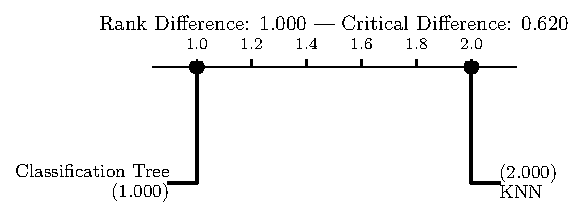
\includegraphics[width=\linewidth]{cd_plot.pdf}
		\caption{Critical difference plot for the $k$-nearest neighbours and classification tree algorithms based on F1-scores.}
		\label{fig:cd}
	\end{figure}
	
	The plots in Figure~\ref{fig:boxplots} represent the box-whisker diagrams for each evaluation metric considered for each models performance on the test set. The classification tree consistently shows better performance for all metrics except the recall metric. The recall for the $k$-NN algorithm is slightly better than the classification tree algorithm, with it having a higher average and tighter dispersion of results. This indicates that the $k$-NN algorithm is slightly better at identifying correct instances across the classes. This provides further evidence that the generalisability performance for the classification tree algorithm on the test dataset is much better than the $k$-NN algorithm
	
	\begin{figure}[hbtp]
		\centering
		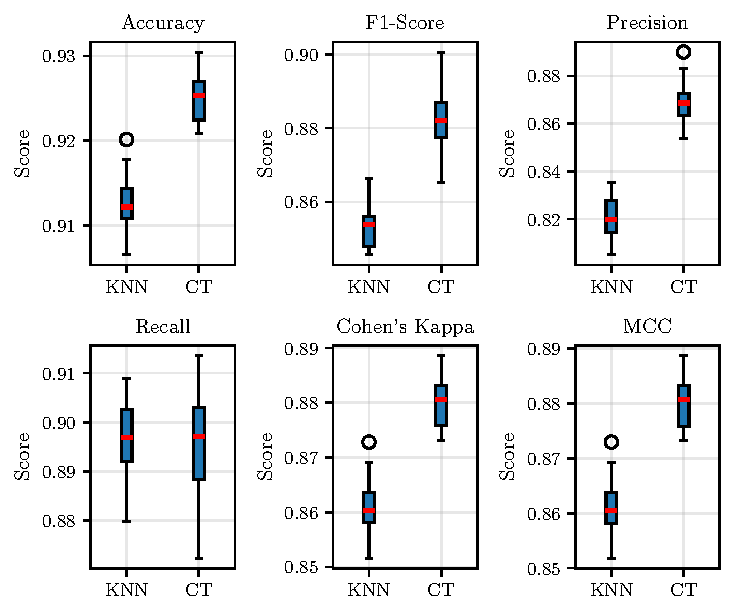
\includegraphics[width=\linewidth]{boxplots.pdf}
		\caption{Box-whisker plots of the evaluation metrics for each algorithms performance on the test dataset.}
		\label{fig:boxplots}
	\end{figure}
	
	Another important aspect to take into consideration when evaluating the two algorithms is the computational complexity. The $k$-NN algorithm is significantly more computationally intensive than classification trees for generating predictions. This is due to the $k$-NN algorithm having to compute multiple distances between new classification points and their nearest neighbours. This is in contrast to the classification tree algorithm which has a computationally expensive training algorithm but generates predictions in real time. As a result of this, real-time analysis and predictions is near impossible for the $k$-NN algorithm. 
	
	\section{Conclusion}\label{C}
	The main objectives of this assignment were to identify and address data quality issues in the forest cover type dataset, develop, implement and optimise $k$-NN and classification tree algorithms, and then determine which approach is best for the forest cover type classification problem. These goals were achieved in this report, through the necessary data pre-processing, the hyper-parameter tuning, the model training, and the comprehensive model evaluation and analysis. 
	
	The forest cover type dataset contains numerous data quality issues including missing values, highly correlated features, noisy features, outliers, features with large numeric ranges, mixed feature types, features with cardinality of one, features with unique values, and skewed class distributions. A targeted implementation of the data pre-processing procedure mitigated the the impact of these data quality issues. The $k$-NN algorithm required more extensive data pre-processing procedures due to its sensitivity to correlated features, noisy features, outliers, features with significantly differing ranges, unique values, and class imbalances. The classification tree algorithm proved to be more robust to these data quality issues and only required pre-processing to mitigate the effect of the target class imbalances. 
	
	The hyper-parameters for each algorithm were tuned using 5-fold cross validation. The $k$-NN algorithm had the highest average cross-validation scores on the training dataset, suggesting that it might have overfit to the training data. The evaluation of the test dataset, split into 20 stratified folds, revealed that the classification tree algorithm had better generalisation performance across multiple metrics. The classification tree algorithm consistently outranked the $k$-NN algorithm for all metrics except for the recall metric. This indicates that the $k$-NN algorithm was marginally better at identifying correct instances across classes. Using the Wilcoxon signed-rank test confirmed that the performance differences between the two algorithms were statistically significant. 
	
	The purpose of this assignment was to explore and understand the fundamental differences between similarity-based and information-based machine learning classification algorithms; to understand the importance of effects that data quality issues and have on each algorithm and how to mitigate these issues with pre-processing techniques and to effectively evaluate the performances of each algorithm across multiple independent runs using different evaluation metrics.
	
	In conclusion, this investigative analysis successfully demonstrated that classification trees are better suited for the forest cover type classification problem. They provide a robust, accurate, and computationally efficient solution.
	
\begin{thebibliography}{00}
	\bibitem{b1} J. D. Kelleher, B. Mac Namee, and A. D’Arcy, \textit{Fundamentals of Machine Learning for Predictive Data Analytics: Algorithms, Worked Examples, and Case Studies}, 2nd ed. Cambridge, MA, USA: The MIT Press, 2020.
	\bibitem{b2} W. McKinney, ``Data structures for statistical computing in Python,'' in \textit{Proceedings of the 9th Python in Science Conference}, S. van der Walt and J. Millman, Eds., 2010, pp. 56--61, doi: 10.25080/Majora-92bf1922-00a.
	\bibitem{b3} F. Pedregosa, G. Varoquaux, A. Gramfort, \textit{et al.}, ``Scikit-learn: Machine learning in Python,'' \textit{Journal of Machine Learning Research}, vol. 12, pp. 2825--2830, 2011.
	\bibitem{b4} C. R. Harris, K. J. Millman, S. J. van der Walt, \textit{et al.}, ``Array programming with NumPy,'' \textit{Nature}, vol. 585, no. 7825, pp. 357--362, Sep. 2020, doi: 10.1038/s41586-020-2649-2.
	\bibitem{b5} G. Lemaître, F. Nogueira, and C. K. Aridas, ``Imbalanced-learn: A Python Toolbox to Tackle the Curse of Imbalanced Datasets in Machine Learning,'' \textit{Journal of Machine Learning Research}, vol. 18, no. 17, pp. 1--5, 2017. [Online]. Available: http://jmlr.org/papers/v18/16-365.html
\end{thebibliography}


	
\end{document}